Remembering chapter~\ref{ch:structure}, it emerged some kind of structure behind data: each tissue seemed to be sampled by a different power law. A topic modelling approach is here proposed. Topic modelling has been developed and studied to approach linguistics problems, so this algorithm was developed considering a network of words and books in input, links represent the abundance of a word in a book. In chapter~\ref{ch:structure}, it was evident that there are many similarities between data considered in this work and linguistics' corpora. Referring to data used in this project \textbf{samples} will be the documents and \textbf{genes} will be the words. It is expected that topics represent some properties of the system due to the gene expression distribution in samples.

The idea is that behind data there are hidden variables that describe the relationship between the genes and the samples. Let's call these variables topics.
Firstly it is necessary to build a bipartite network of genes and samples, then nodes are linked considering the gene expression value in the dataset.
\begin{figure}[htb!]
    \centering
    \includegraphics[width=0.7\linewidth]{pictures/topic/bipartite.pdf}
    \caption{An example of a bipartite network. Samples are on the left, genes are on the right. Each link is weighted by gene expression value. On the left side, all nodes of the same colour are clusters of samples. On the right side, all nodes with the same colour are a set of genes, also known as topics.\\
    Blue lines represent the cluster structure, each blue squared-dot is a set of nodes, lines delineate the hierarchical structure.\\
    It is clear, in the middle, the network separation between genes and samples.}
    \label{fig:topic/bipartite}
\end{figure}

The output of this kind of models consists of sets of genes, the topics, with a probability distribution $P(\text{gene} | \text{topic})$ and probability distributions of these topics inside each sample $P(\text{topic} | \text{sample})$, together they give the relationship between a \textit{sample} and a \textit{gene}.

In this work, an innovative and recent approach to topic model is proposed. The algorithm was presented by~\cite{gerlach2018network} and~\cite{Peixoto2017} explained it in details. This model is an evolution of a stochastic block model~\cite{Holland1983}. It is called hierarchical Stochastic Block Model (hSBM).

The ultimate goal is being able to separate healthy and diseased samples, then find and separate well-known tumour types and finally extend the actual knowledge and retrieve the tumour sub-types.

One of the advantages of this particular algorithm is that it is hierarchical, so it applies community detection at different layers of resolution. So the output has got different resolutions and a different number of clusters at each layer. One extreme layer is, by definition, the one which separates genes ($\simeq$ words) and samples ($\simeq$ samples) in two blocks. In the other layers, it is possible to have few big clusters until the other extreme were the number of clusters is comparable with the number of nodes.
\begin{figure}[htb!]
  \centering
  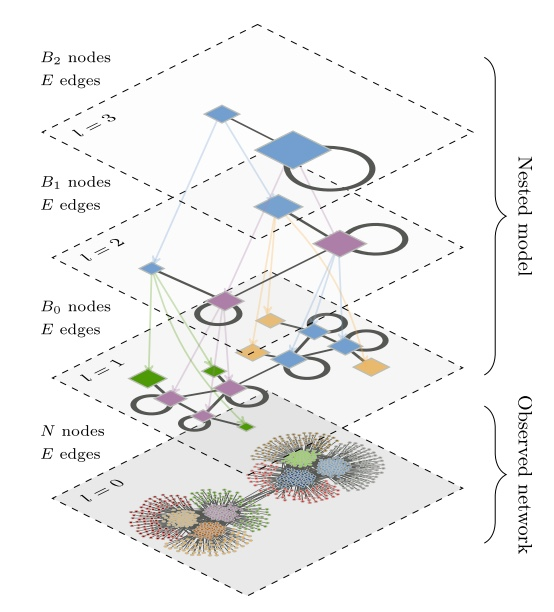
\includegraphics[width=0.6\linewidth]{pictures/topic/peixioto_hierarchic.jpg}
  \caption{Example of a hierarchical structure. At $l=0$ the number of cluster is comparable with the number of nodes, is the situation with many small clusters. Then they're merged in bigger clusters at other layers of the hierarchy.}
  \label{fig:topic_peixioto_hierarchic}
\end{figure}

What the algorithm does is to run a sort of Monte Carlo simulation and find the best partition of the data.
The probability that the hidden variables $\theta$ describe the data $G$ $P(\theta | G)$ can be written as a likelihood times a prior probability as
\[P(\theta|G)=\frac{P(G|\theta)\overbrace{P(\theta)}^{prior}}{\underbrace{P(G)}_{\sum_{\theta}P(G|\theta)P(\theta)}}.\]
It is possible to define a description length
\[
\Sigma=-lnP(G|\theta)-lnP(\theta),
\]
so that $P(\theta | G)\propto e^{-\Sigma}$.
Moreover, the likelihood $P(G | \theta)$, can be written as $\frac{1}{\Omega}$ where $\Omega(\theta)$ is the number of networks that is possible to build given $\theta$. This corresponds to a microcanonical ensemble with entropy $S=Ln\left(\Omega\right)$. According to~\cite{peixoto2017nonparametric} entropy $S$ can be written as
\[
S=\frac{1}{2}\Sigma_{r,s} n_r n_s H\left(\frac{e_{rs}}{n_rn_s}\right),
\]
where $n_r$ is the number of nodes in the block $r$, $e_{rs}$ the number of links between nodes of group $r$ and nodes of group $s$ and $H$ is the Shannon entropy $H(x)=xLog_2(x)+(1-x)Log_2(1-x)$. Note that $S$ is minimal if $\frac{e_{rs}}{n_rn_s}$ is close to zero, $r$ and $s$ are two completely separated blocks or if it is close to $1$, $r$ and $s$ are groups with many connections; this allows finding groups with nodes very disconnected or topic and clusters with a lot of connections. Note that the description length of a network's state is related to the entropy of the states' ensemble:
\[
\Sigma=S-lnP(\theta).
\]
The algorithm tries to minimize $S$, so that $\Sigma$ is minimized, so $e^{-\Sigma}$ is maximized, but this is $P(\theta | G)$ that is the required probability to maximize.

The Monte Carlo simulation works in a few steps:
\begin{itemize}
 \item a node $i$ is chosen,
 \item the group of $i$ is called $r$,
  \item a node $j$ is chosen from $i$'s neighbours, the group of $j$ is called $t$,
  \item a random group $s$ is selected,
  \item move of node $i$ to group $s$ is accepted with probability $P(r\to s|t)=\frac{e_{ts}+\epsilon}{e_t+\epsilon B}$,
  \item if the move to $s$ is not accepted, a random edge $e$ is chosen from group $t$ and node $i$ is assigned to the endpoint of $e$ which is not in $t$;
\end{itemize}
in figure~\ref{fig:topic_peixioto_move} an example of these steps.
\begin{figure}[htb!]
  \centering
  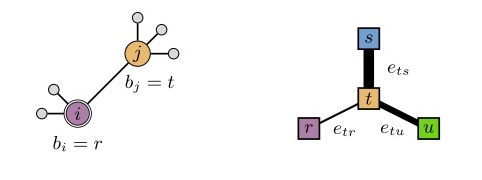
\includegraphics[width=0.9\linewidth]{pictures/topic/peixioto_move.jpg}
  \caption{Left: Local neighbourhood of node $i$ belonging to block $r$, and a randomly chosen neighbour $j$ \
  belonging to block $t$. \
  Right: Block multi-graph, indicating the number of edges between blocks, represented as the edge thickness. \
  In this example, the attempted move $bi \to s$ is made with a larger probability than either $bi \to u$\
   or $bi \to r$ (no movement), since $e_{ts}>e_{tu}$ and $e_{ts}>e_{tr}$.}
  \label{fig:topic_peixioto_move}
\end{figure}

In order to remove eventual biases due to the initial configuration the model is run with $5$ different initial states, then the final state with the minimal entropy is selected.

Once the model runned, it is possible to estimate the probability distribution of words inside a topic
\[P(w|t_w)=\frac{\text{\# of edges on $w$ to $t_w$}}{\text{\# of edges on $t_w$}}\]
and the topic distribution inside a document
\[P(t_w|d)=\frac{\text{\# of edges on $d$ from $t_w$}}{\text{\# of edges on $d$}}.\]
This algorithm can be set to accept overlapping partitions; in this case, the presence of a word in a topic is not trivial and can be estimated as
\[P(t_w|w)=\frac{\text{\# of edges on $w$ to $t_w$}}{\text{\# of edges on $w$}}.\]
The membership of a document in a cluster is
\[P(t_d|d)=\frac{\text{\# of edges on $d$ to $t_d$}}{\text{\# of edges on $d$}}.\]

See appendix~\ref{app:hsbm} for a detailed analysis of the maths behind the algorithm and \url{https://hub.docker.com/r/fvalle01/hsbm} for the extension of~\cite{gerlach2018network} to non-linguistics component systems datasets.
